\subsection{Misura finale}

In base all'esperienza acquisita nella parte ``di calibrazione'',
e in base ai limiti di moduli NIM disponibili e tempo rimasto,
abbiamo effettuato quattro tipi di misure ``ufficiali'' con cui calcolare il flusso di muoni.
Per queste misure abbiamo coperto l'apparato dalla luce
con un telo nero, un laminato di plastica e un'amaca.

\begin{figure}
	\centering
	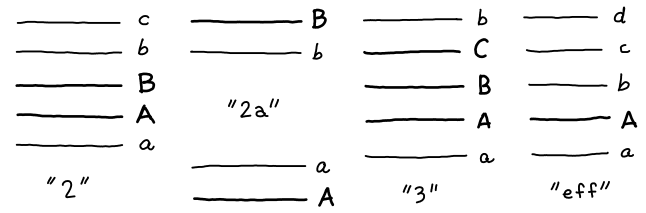
\includegraphics[width=30em]{modmisfinale}
	\caption{\label{fig:modmisfinale}
	Schema dei tipi di misura usati per il fit finale.
	Le linee orizzontali rappresentano le lastre di scintillatore;
	le lettere maiuscole indicano le lastre il cui conteggio in coincidenza
	viene usato per misurare il flusso (fa eccezione la configurazione ``eff''),
	le lettere minuscole indicano le lastre usate per misurare l'efficienza
	di quelle con le lettere maiuscole.}
\end{figure}

\subsubsection{Misure in coincidenza a 2}

\begin{figure}
	\centering
	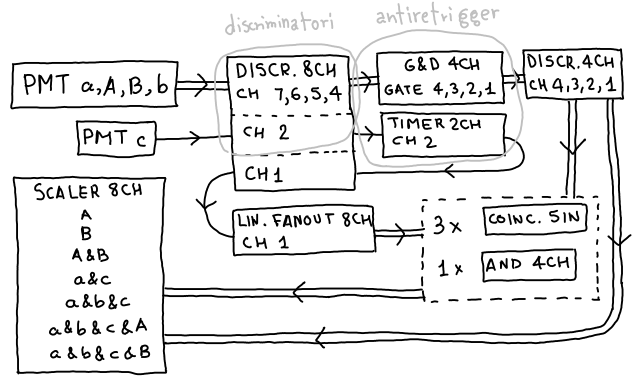
\includegraphics[width=30em]{circuitomisdue}
	\caption{\label{fig:circuitomisdue}
	Circuito per la misura in configurazione ``2''.
	Le linee di collegamento doppie rappresentano genericamente più di un cavo.
	I segnali dei PMT vanno ai discriminatori.
	Dopo i discriminatori ci sono i moduli \texttt{Gate\&Delay} e \texttt{Dual Timer}
	impostati su una durata di \SI{700}{ns} non retriggerabile;
	i segnali di questi passano da discriminatori <<secondo stadio>> (per distinguerli dagli altri)
	che riportano la durata dei segnali a circa~\SI{40}{ns}.}
\end{figure}

Usiamo il conteggio di due lastre (chiamate $A$ e $B$) in coincidenza per misurare il flusso
e tre lastre in coincidenza ($a$, $b$ e $c$) per misurare le efficienze di $A$ e $B$
(vedi configurazione ``2'' in \autoref{fig:modmisfinale}).
Usare solo due lastre in coincidenza ci permette di scegliere le lastre più vicine possibili nel nostro apparato
e quindi di avere l'accettanza geometrica maggiore possibile.
Usiamo altre tre lastre per l'efficienza anziché due in modo da non doverci preoccupare del rumore.
Le lastre $A$ e $B$ sono comprese tra le lastre $a$, $b$ e $c$
in modo che la misura dell'efficienza non dipenda dalla distribuzione angolare.
Complessivamente quindi questa misura è ottimizzata per il flusso totale.

Il circuito è riportato in \autoref{fig:circuitomisdue}.
I circuiti delle altre configurazioni sono in sostanza uguali.

\subsubsection{Misure in coincidenza a 2 con distribuzione angolare}

\begin{table}
	% \centering
	\small
	\hspace{-5em}
	\begin{tabular}{ll|lrrrrrrr|c}
		sogliaA & sogliaB & clock & A & B & A\&B & a\&b & a\&b\&B & a\&b\&A & a\&b\&A\&B & prefit \\
		\hline
		307.3 & 297.3 & 1e5 & 1008979 & 270259 & 920 & 1763 & 1224 & 702 & 555  & 1               \\
		307.3 & 297.3 & 1e6 & 9995686 & 2690915 & 9059 & 17919 & 12177 & 6977 & 5346 & 0          \\
		1468 & 1832 & 1e5 & 98858 & 92615 & 601 & 1859 & 1221 & 688 & 509  & 1                    \\
		1468 & 1832 & 1e6 & 988694 & 926201 & 5550 & 17807 & 11758 & 6195 & 4645 & 0              \\
		1.287e3 & 0.964e3 & 1e5 & 197923 & 205786 & 634 & 1708 & 1160 & 615 & 487  & 1            \\
		1.287e3 & 0.964e3 & 1e6 & 1996164 & 2070802 & 6443 & 17532 & 11819 & 6397 & 4922 & 0      
	\end{tabular}
	\caption{\label{tab:data2a}
	Dati per la misura finale in configurazione ``2a''.
	La notazione è la stessa della \autoref{tab:data2}.
	Tutte le misure sono state fatte con $A$ = PM1, $B$ = PM6, $a$ = PM2, $b$ = PM5.
	L'alimentazione di $A$ e $B$ è \SI{2000}V.
	Le durate del secondo stadio sono le stesse della configurazione ``2''.}
\end{table}

Questa configurazione (``2a'' in \autoref{fig:modmisfinale}) è simile alla precedente,
ma le lastre usate per misurare l'efficienza sono comprese tra quelle usate per misurare il flusso anziché esterne.
Questo ci permette di scegliere le lastre $A$ e $B$ il più lontane possibile
in modo da essere particolarmente sensibili alla densità verticale di raggi.
Le due lastre aggiuntive sono comunque disposte in modo da minimizzare
la dipendenza dall'accettanza della misura di efficienza.
Le lastre aggiuntive sono due ($a$ e $b$) anziché tre
perché usiamo anche $B$ per misurare l'efficienza di $A$ e viceversa.

\subsubsection{Misure in coincidenza a 3}

\begin{table}
	\small
	\hspace{-9em}
	\begin{tabular}{lll|rrrrrrrr|c}
		sogliaA & sogliaB & sogliaC & clock & C & B & A\&B\&C & a\&b & a\&b\&C & a\&b\&B & a\&b\&A & prefit \\
		\hline
		307.1 & 297.1 & 207.1 & 53093476 & 62962492 & 723662210 & 1073466 & 668411 & 617769 & 607441 & 591279 & 0
	\end{tabular}
	\caption{\label{tab:data3}
	Dati per la misura finale in configurazione ``3''.
	La notazione è la stessa della \autoref{tab:data2}.
	Le tensioni di alimentazione di $A$ e $B$ sono \SI{2000}V.
	Le etichette sono $A$ = PM3, $B$ = PM4, $C$ = PM5, $a$ = PM2, $b$ = PM6.
	Le durate del secondo stadio per $A$ e $B$ sono le stesse della configurazione ``2''.
	Il secondo stadio di $a$, $b$ e $C$ è \SI{35\pm1}{ns}.
	Sono stati misurati separatamente i tassi di $A$, $a$ e $b$:
	su un clock di 1e5, i conteggi sono $C_A=4243753$, $C_a=86130$, $C_b=31799$.}
\end{table}

In questa configurazione (``3'' in \autoref{fig:modmisfinale})
usiamo tre lastre ($A$, $B$ e $C$) in coincidenza per misurare il flusso
e due lastre ($a$ e $b$) esterne ad $A$, $B$ e $C$ per misurare l'efficienza di $A$, $B$ e $C$.
In questo modo non dobbiamo preoccuparci del rumore sulle lastre con cui misuriamo il flusso.
È interessante confrontare questa misura con una della configurazione ``2'' tale che $A_2=A_3$ e $B_2=C_3$.

\subsubsection{Misure di efficienza con distribuzione angolare}

\begin{table}
	\small
	\hspace{-10.5em}
	\begin{tabular}{l|rrrrrrrr|ccccc|c}
		sogliaA & clock & A &a\&b & a\&b\&A & b\&c & b\&c\&A & b\&d & b\&d\&A & PMA & PMa & PMb & PMc & PMd & prefit \\
		\hline\hline
		2216 & 1e5   & 2862828 & 1989 & 1791 & 2630 & 1830 & 1908 & 1402 & 3 & 2 & 4 & 5 & 6 & 1           \\
		2216 & 1e6   & 29620183 & 19040 & 17372 & 26445 & 18041 & 18864 & 13703 & 3 & 2 & 4 & 5 & 6 & 0     \\
		5.11e3 & 1e5 & 120032 & 1975 & 1782 & 2684 & 1804 & 1888 & 1362 & 3 & 2 & 4 & 5 & 6 & 1         \\
		306.5 & 1e5  & 4464209 & 1957 & 1790 & 2641 & 1833 & 1926 & 1421 & 3 & 2 & 4 & 5 & 6 & 1          \\
		\hline
		306.5 & 1e5  & 122838 & 965 & 922 & 2500 & 1847 & 1938 & 1443 & 2 & 1 & 3 & 4 & 5 & 1            \\
		306.5 & 1e6  & 1239854 & 9576 & 9163 & 24663 & 18227 & 19352 & 14530 & 2 & 1 & 3 & 4 & 5 & 0      \\
		1460 & 1e5   & 104482 & 955 & 903 & 2465 & 1773 & 1961 & 1443 & 2 & 1 & 3 & 4 & 5 & 1             \\
		\hline
		1460 & 1e5   & 50512 & 943 & 901 & 2465 & 1802 & 1454 & 1088 & 2 & 1 & 3 & 4 & 6 & 0             
	\end{tabular}
	\caption{\label{tab:dataeff}
	Dati per la misura finale in configurazione ``eff''.
	La notazione è la stessa della \autoref{tab:data2}.
	Le alimentazioni sono
	$V_1=\SI{2000}V$, $V_2=\SI{2000}V$, $V_3=\SI{1900}V$, $V_4=\SI{1950}V$, $V_5=\SI{2000}V$, $V_6=\SI{2000}V$,
	ad eccezione di $A$ che è sempre a \SI{2000}V.
	I~rate di $a$, $b$, $c$, $d$ sono sempre circa \SI{500}{s^{-1}}.}
\end{table}

Questa configurazione (``eff'' in \autoref{fig:modmisfinale})
è abbastanza diversa dalle altre perché è ottimizzata per la distribuzione angolare anziché per il flusso.
Misuriamo l'efficienza di una lastra $A$ con varie coppie delle lastre $a$, $b$, $c$, $d$.
Imponendo che l'efficienza di $A$ sia la stessa e scegliendo in modo opportuno le coppie
si ottiene un forte vincolo sulla distribuzione angolare dei raggi.
Delle lastre minuscole almeno una è dal lato opposto di $A$ rispetto alle altre in modo
da avere almeno una misura di efficienza che non dipende dalla distribuzione angolare.

\subsection{Fit}


% l'ambiente {landscape} gira la pagina in orizzontale quando la vedi a schermo e la lascia verticale quando stampi.
\begin{landscape}
	\begin{table}[p]
		\centering
		\small
		\begin{tabular}{llll|lrrrrrrr|ccccc|c}
			sogliaA & sogliaB & alimA & alimB & clock & A & B & A\&B & a\&c & a\&b\&c & a\&b\&c\&A & a\&b\&c\&B & PMA & PMB & PMa & PMb & PMc & prefit \\
			\hline\hline
			5.97e3 & 10.14e3 & 1900 & 1900 & 1e5 & 7513 & 16958 & 1632 & 1140 & 1054 & 764 & 842 & 3 & 4 & 2 & 5 & 6 & 1                          \\
			5.97e3 & 10.14e3 & 1900 & 1900 & 3e5 & 22504 & 50217 & 4923 & 3677 & 3405 & 2426 & 2748 & 3 & 4 & 2 & 5 & 6 & 1                       \\
			5.97e3 & 10.14e3 & 2000 & 2000 & 1e5 & 23688 & 89514 & 2286 & 1200 & 1110 & 1005 & 1049 & 3 & 4 & 2 & 5 & 6 & 1                       \\
			5.97e3 & 10.14e3 & 2000 & 2000 & 1e5 & 24057 & 85104 & 2317 & 1293 & 1207 & 1081 & 1115 & 3 & 4 & 2 & 5 & 6 & 1                       \\
			4.71e3 & 10.14e3 & 2000 & 2000 & 1e5 & 85713 & 84140 & 2391 & 1241 & 1149 & 1044 & 1071 & 3 & 4 & 2 & 5 & 6 & 1                       \\
			3.98e3 & 6.28e3 & 2000 & 2000 & 1e5 & 336320 & 337053 & 2699 & 1238 & 1141 & 1042 & 1079 & 3 & 4 & 2 & 5 & 6 & 1                      \\
			3.98e3 & 6.28e3 & 2000 & 2000 & 1e5 & 347229 & 339499 & 2678 & 1272 & 1150 & 1054 & 1098 & 3 & 4 & 2 & 5 & 6 & 1                      \\
			3.98e3 & 6.28e3 & 2000 & 2000 & 1e6 & 3486673 & 3654718 & 26777 & 12175 & 11163 & 10307 & 10608 & 3 & 4 & 2 & 5 & 6 & 0               \\
			4.47e3 & 7.93e3 & 2000 & 2000 & 54413944 & 93555166 & 107266650 & 1370413 & 675409 & 620744 & 567583 & 586641 & 3 & 4 & 2 & 5 & 6 & 0 \\
			4.47e3 & 7.93e3 & 2000 & 2000 & 5428946 & 12407950 & 15049021 & 141548 & 67278 & 61960 & 56592 & 58785 & 3 & 4 & 2 & 5 & 6 & 0        \\
			\hline
			4.47e3 & 297.2 & 2000 & 2000 & 1e5 & 218729 & 116204 & 2074 & 1247 & 1136 & 1048 & 1098 & 3 & 5 & 2 & 4 & 6 & 1                       \\
			4.47e3 & 297.2 & 2000 & 2000 & 74832702 & 98917344 & 88277251 & 1550323 & 928983 & 847036 & 783834 & 826330 & 3 & 5 & 2 & 4 & 6 & 0   \\
			4.47e3 & 297.2 & 2000 & 2000 & 1e5 & 335083 & 204463 & 2061 & 1249 & 1120 & 1037 & 1095 & 3 & 5 & 2 & 4 & 6 & 1    \\   %   senza telo nero 
			765 & 297.2 & 2000 & 2000 & 1e5 & 4134344 & 187105 & 2838 & 1268 & 1159 & 1076 & 1100 & 3 & 5 & 2 & 4 & 6 & 1      \\   %  senza telo nero  
			307.3 & 297.2 & 2000 & 2000 & 1e5 & 4426281 & 186124 & 3000 & 1256 & 1117 & 1039 & 1068 & 3 & 5 & 2 & 4 & 6 & 0     \\  %  # senza telo nero
			\hline
			307.3 & 297.2 & 2000 & 2000 & 1e5 & 120570 & 97688 & 1867 & 522 & 480 & 458 & 463 & 2 & 5 & 1 & 4 & 6 & 1                             \\
			307.3 & 297.2 & 2000 & 2000 & 1e6 & 1206351 & 977575 & 19370 & 5387 & 4949 & 4749 & 4808 & 2 & 5 & 1 & 4 & 6 & 0                      \\
			\hline
			% forse le due prossime due misure avranno qualcosa che non va
			% -> confermo dal prefit che sono molto sballate anche supponendo che i raggi siano verticali
			% 307.3 & 297.2 & 2000 & 2000 & 1e5 & 121504 & 253216 & 1574 & 680 & 603 & 570 & 472 & 2 & 6 & 1 & 4 & 5 & 1
			% 307.3 & 1.517e3 & 2000 & 2000 & 1e5 & 122622 & 131362 & 1467 & 756 & 720 & 641 & 528 & 2 & 6 & 1 & 4 & 5 & 1
			307.3 & 1.517e3 & 2000 & 2000 & 1e6 & 1233265 & 1329361 & 14334 & 7256 & 6400 & 6056 & 4909 & 2 & 6 & 1 & 4 & 5 & 0                   \\
			307.3 & 1.517e3 & 2000 & 2000 & 1e5 & 122701 & 134106 & 1480 & 751 & 676 & 646 & 532 & 2 & 6 & 1 & 4 & 5 & 1                          \\
			307.3 & 297.3 & 2000 & 2000 & 1e5 & 122750 & 253274 & 1492 & 687 & 605 & 567 & 477 & 2 & 6 & 1 & 4 & 5 & 0                            \\
			\hline
			307.3 & 297.3 & 2000 & 2000 & 1e5 & 125673 & 111377 & 1971 & 538 & 493 & 466 & 482 & 2 & 5 & 1 & 4 & 6 & 1                            \\
			307.3 & 297.3 & 2000 & 2000 & 12840754 & 13958014 & 14572786 & 255165 & 68855 & 63402 & 60630 & 62120 & 2 & 5 & 1 & 4 & 6 & 0         
		\end{tabular}
		\caption{\label{tab:data2}
		Dati per la configurazione ``2'' della misura finale.
		I dati sono riportati in ordine cronologico di acquisizione.
		Le colonne <<soglia\dots>> riportano la soglia del discriminatore in decimillesimi di volt.
		Le colonne <<alim\dots>> riportano la tensione nominale di alimentazione dei PMT in volt.
		La colonna <<clock>> riporta il conteggio del \texttt{clock} del contatore,
		quindi il tempo di acquisizione in millesimi di secondo.
		Le colonne successive a <<clock>> sono i conteggi; le <<\&>> indicano le coincidenze.
		Le colonne <<PM\dots>> indicano a quali PM corrispondono le etichette $A$, $B$, $a$, $b$, $c$;
		le linee orizzontali nella tabella demarcano il cambiamento degli assegnamenti.
		La colonna <<prefit>> indica se i dati vengono utilizzati nel fit preliminare (1) o nel fit finale (0).
		Le durate dei discriminatori secondo stadio (vedi circuito in \autoref{fig:circuitomisdue})
		sono \SI{38\pm2}{ns} per $A$ e \SI{37\pm2}{ns} per $B$.
		Il secondo stadio di $a$, $b$ e $c$ è a circa \SI{40}{ns}.}
	\end{table}
\end{landscape}
